\documentclass{article}

\usepackage{polski}
\usepackage[utf8]{inputenc}
\usepackage{booktabs}
\usepackage{biblatex}

\usepackage{graphicx}
\usepackage{float}
\usepackage{geometry}
\usepackage{listings}
\geometry{
	a4paper,
	total={170mm,257mm},
	left=50mm,
	right=50mm,
	top=45mm,
	bottom = 45mm
}
\usepackage{tabularx}


\begin{document}
	\newgeometry{tmargin=4cm, bmargin=4cm, lmargin=3cm, rmargin=3cm}
	
	\begin{titlepage}
		\center
		\newcommand{\HRule}{\rule{\linewidth}{0.6mm}}
		
		\textsc{\LARGE Politechnika Wrocławska}\\[1.5cm]
		\textsc{\Large Laboratorium}\\[0.5cm] 
		\textsc{\large Inteligencja Obliczeniowa i jej Zastosowania}\\[0.7cm] 

		\HRule \\[0.4cm]
		{ \huge \bfseries Algorytmy ewolucyjne i hybrydowe}\\[0.4cm]
		\HRule \\[1.5cm]
		
		\begin{minipage}{0.4\textwidth}
			\begin{flushleft} \large
				\emph{Authors:}\\
				Rafał \textsc{Pieniążek}\\
                Jakub \textsc{Pomykała}
			\end{flushleft}
		\end{minipage}
		~
		\begin{minipage}{0.4\textwidth}
			\begin{flushright} \large
				\emph{Supervisor:} \\
				prof. dr inż. Olgierd \textsc{Unold} 
			\end{flushright}
		\end{minipage}\\[4cm]

		{\large \today}\\[3cm]
		
		\vfill
		
	\end{titlepage}


\newpage
\section{Wstęp}
	Celem laboratorium było przeprowadzenie optymalizacji globalnej dla wybranych funkcji z pakietu globalOptTests.
    


\section{Funkcja Aluffi - Pentini}
	\subsection{Wzór analityczny}
	   \begin{figure}[!htbp]
    \centering
    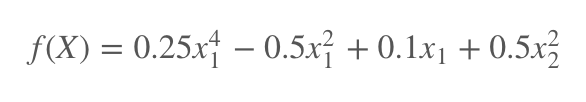
\includegraphics[width=0.7\textwidth]{inc/wzory/aluffi-pentini}
     \caption{Wzór analityczny funkcji Aluffi - Pentini}
    \end{figure}
    
    \subsection{Wykres w ustalonym przedziale zmiennych}
    
    
    \subsection{Optymalizacja poszukiwania ekstremum globalnego}
    
\section{Funkcja Branina}
\subsection{Wzór analityczny}
\begin{figure}[!htbp]
    \centering
    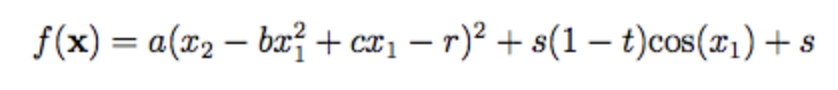
\includegraphics[width=0.7\textwidth]{inc/wzory/branin}
     \caption{Wzór analityczny funkcji Branina}
    \end{figure}
\section{Funkcja Bohachevsky'ego}
\subsection{Wzór analityczny}
\begin{figure}[!htbp]
    \centering
    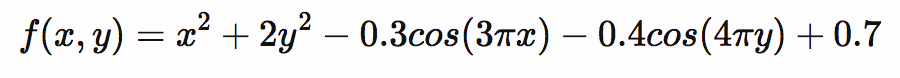
\includegraphics[width=0.7\textwidth]{inc/wzory/bohachevsky}
     \caption{Wzór analityczny funkcji Bochachevsky'ego}
    \end{figure}
\section{Wnioski}

\end{document}\documentclass{article}